%=====================================================================
%  Abbes — 18-DOF Humanoid Robot : End-of-Studies Project Report
%  Main file.  Compile with:  latexmk -pdf main.tex
%=====================================================================
\documentclass[12pt,a4paper,oneside]{report}

%--------------------- Encoding & language ---------------------------
\usepackage[utf8]{inputenc}
\usepackage[T1]{fontenc}
\usepackage{lmodern}
\usepackage[english]{babel}
\usepackage{textcomp}
\providecommand{\euro}{\texteuro}

%--------------------- Page geometry ---------------------------------
\usepackage[a4paper,margin=2.5cm]{geometry}

%--------------------- Graphics & color ------------------------------
\usepackage{graphicx}
\usepackage{xcolor}
\usepackage{caption}
\usepackage{subcaption}
\usepackage{tikz}
\usetikzlibrary{positioning,arrows.meta,shapes.geometric,fit,backgrounds,calc}
\graphicspath{{figures/}}

%--------------------- Math, tables, lists ---------------------------
\usepackage{amsmath,amssymb}
\usepackage{booktabs}        % professional tables (\toprule \midrule \bottomrule)
\usepackage{array}
\usepackage{tabularx}        % auto-width columns
\usepackage{enumitem}        % tighter list control

%--------------------- Source-code listings --------------------------
\usepackage{listings}
\lstdefinestyle{cpp}{
  language=C++,
  basicstyle=\ttfamily\footnotesize,
  keywordstyle=\color{blue!60!black}\bfseries,
  commentstyle=\color{green!35!black}\itshape,
  stringstyle=\color{purple!70!black},
  numbers=left, numberstyle=\tiny\color{gray}, numbersep=7pt,
  frame=single, rulecolor=\color{gray!40},
  backgroundcolor=\color{gray!4},
  breaklines=true, showstringspaces=false, tabsize=2,
  columns=flexible, captionpos=b, xleftmargin=14pt,
}
\lstset{style=cpp}

%--------------------- Misc layout helpers ---------------------------
\usepackage{setspace}
\usepackage{ulem}\normalem   % for \uline (underline) without italicising everything

%--------------------- Cross-refs & links (load last) ----------------
\usepackage[hidelinks]{hyperref}

%=====================================================================
%  COVER-PAGE CONFIGURATION  --  *** EDIT THESE VALUES ***
%=====================================================================
\newcommand{\projType}{Projet Personnel Professionnel}
\newcommand{\projSpeciality}{Software Engineering}
\newcommand{\projLevel}{3rd Year Engineering}
\newcommand{\projTitle}{Design and Software Architecture of an 18-DOF
  Humanoid Robot: ROS\,2 Control, Simulation and an LLM-Based
  Natural-Language Command Layer}
\newcommand{\projAuthorA}{Zeyneb Benabdallah}
\newcommand{\projAuthorB}{Yassine Allouch}
\newcommand{\projSupervisor}{Mme Hajer Taktak}
\newcommand{\projDefDate}{03/06/2026}
\newcommand{\projYear}{2025\,/\,2026}
%=====================================================================

\begin{document}

  %=====================================================================
%  Cover page  (layout modelled on the reference PFA cover)
%=====================================================================
\begin{titlepage}
\centering

%--------------------- Top header: logos + institution --------------
\noindent
\begin{minipage}[c]{0.25\textwidth}
  \centering
  
\includegraphics[width=\linewidth]{logo_carthage.png}
\end{minipage}%
\hfill
\begin{minipage}[c]{0.46\textwidth}
  \centering
  Ministry of Higher Education\\
  and Scientific Research\\
  *** * ***\\
  University of Carthage\\
  *** * ***\\
  \textbf{National Institute\\
  of Applied Science and\\
  Technology}
\end{minipage}%
\hfill
\begin{minipage}[c]{0.22\textwidth}
  \centering
  
\includegraphics[width=\linewidth]{logo_insat.png}
\end{minipage}

\vspace{0.6em}
\noindent\rule{\textwidth}{0.8pt}

%--------------------- Project type / speciality / level ------------
\vspace{2.2em}
{\scshape\LARGE \projType\par}
\vspace{1.6em}
{\scshape\Large Speciality: \projSpeciality\par}
\vspace{1.0em}
{\scshape\Large Level: \projLevel\par}
\vspace{2.2em}

\noindent\rule{\textwidth}{0.8pt}

%--------------------- Topic / title --------------------------------
\vspace{1.6em}
{\uline{\textbf{Topic:}}\par}
\vspace{1.2em}
{\bfseries\Large \projTitle\par}
\vspace{1.6em}

\noindent\rule{\textwidth}{0.8pt}

%--------------------- Author / supervisor --------------------------
\vspace{2.6em}
{\itshape Prepared by:\par}
\vspace{0.4em}
{\bfseries\itshape\large \projAuthorA\par}
\vspace{0.3em}
{\bfseries\itshape\large \projAuthorB\par}

\vspace{1.8em}
{\itshape Supervisor:\par}
\vspace{0.4em}
{\bfseries\itshape\large \projSupervisor\par}

\vspace{1.8em}
{\itshape\small Defended on \projDefDate\par}

\vspace{1.4em}
{\large School Year: \projYear\par}

\vfill
\end{titlepage}


\pagenumbering{roman}
%=====================================================================
%  Acknowledgements   (draft text -- edit freely)
%=====================================================================
\chapter*{Acknowledgements}
\addcontentsline{toc}{chapter}{Acknowledgements}

This work could not have been accomplished without the support and
guidance of many people, to whom the authors wish to express their
sincere gratitude.

The authors address their thanks first of all to their supervisor,
\textbf{\projSupervisor}, for the trust she placed in them, for her
guidance, her valuable advice and her availability throughout this
project. Her insight greatly shaped both the technical direction and
the quality of this work.

The authors also extend their gratitude to the members of the jury for
the honour of agreeing to evaluate this project, as well as to the
teaching staff of the \emph{National Institute of Applied Science and
Technology (INSAT)} for the knowledge shared throughout their studies.

Finally, the authors warmly thank their families and friends for their
constant encouragement and unwavering support throughout this journey.

%=====================================================================
%  Abstract   (draft text -- edit freely)
%=====================================================================
\chapter*{Abstract}
\addcontentsline{toc}{chapter}{Abstract}

This report presents the design and software architecture of
\textbf{Abbes}, a child-sized, 3D-printed humanoid robot with eighteen
degrees of freedom (18-DOF). The platform is built end to end: from the
mechanical CAD model and the electronics organised around an ESP32
micro-ros node, to a complete ROS\,2 software stack that handles
kinematics, balance and bipedal-gait generation. A Gazebo simulation
provides a digital twin used for validation before deployment on the
physical robot. Beyond the classical motion-control pipeline, the
project introduces a high-level \emph{natural-language command layer}:
a locally hosted Large Language Model grounds free-form user
instructions into a fixed, safety-checked command vocabulary that
drives the robot's actions. Particular emphasis is placed on the
software engineering aspects of the system --- the embedded firmware,
the ROS\,2 control architecture and the artificial-intelligence command
pipeline --- while the mechatronic and gait-planning foundations of the
platform are also covered.


\tableofcontents
\listoffigures
\listoftables
\cleardoublepage

\pagenumbering{arabic}

% ---- Chapters (added part by part) ----
%=====================================================================
%  Chapter 1 — General Presentation and State of the Art
%=====================================================================
\chapter{General Presentation and State of the Art}
\label{chap:presentation}

\section{Introduction}

Humanoid robotics is one of the most demanding fields of modern
engineering: it combines mechanical design, real-time control, embedded
electronics, and, increasingly, artificial intelligence into a single
integrated system. Reproducing a behaviour as ordinary as human walking
requires a machine to balance on a small support area while continuously
coordinating many actuators, all under strict timing constraints. This
makes a humanoid platform an ideal testbed for studying the interaction
between low-level real-time control and high-level decision making.

This chapter introduces the project by outlining its objectives and its
significance in the field of bipedal robotics. It then discusses the
problematic aspects associated with bipedal walking, presents the state
of the art through a few representative humanoid robots, and finally
positions the \textbf{Abbes} robot --- the platform developed in this
work --- with respect to those references. The objectives pursued are:

\begin{enumerate}[itemsep=2pt,topsep=4pt]
  \item Design and assemble an 18-DOF humanoid structure from 3D-printed
        parts driven by hobby servo-motors.
  \item Implement the on-board real-time firmware that actuates the
        joints and streams inertial measurements.
  \item Build a modular ROS\,2 software stack covering the kinematic
        model, balance control, and bipedal-gait generation.
  \item Validate the robot in a physics-based simulation (digital twin)
        before deployment on hardware.
  \item Add a natural-language command layer, based on a locally hosted
        Large Language Model, that translates free-form user requests
        into a fixed and safety-checked set of robot actions.
\end{enumerate}

\section{Problematic}
\label{sec:problematic}

Bipedal walking poses a unique set of challenges that stem from the need
to maintain dynamic stability on two legs. For the platform developed
here, these challenges are tightly coupled with the software-engineering
goals of the project. The core problematic aspects are:

\begin{itemize}[itemsep=2pt,topsep=4pt]
  \item \textbf{Mechanical design.} Defining a joint distribution that
        is rich enough to produce a stable, human-like gait while
        remaining buildable with low-cost, 3D-printed parts and hobby
        servo-motors.
  \item \textbf{Control system.} Despite the need for inverse kinematics
        in controlling a walking humanoid, ensuring robustness and
        adaptability in real-time control algorithms running on a
        resource-constrained microcontroller remains a significant
        challenge.
  \item \textbf{Stability criteria.} Keeping the robot balanced during
        the various phases of walking, which requires a recognised
        stability criterion and an inertial feedback loop.
  \item \textbf{ROS\,2 integration.} Leveraging the advanced integration
        capabilities of ROS\,2 to bridge a physics-based simulation and
        the physical robot through a common middleware.
  \item \textbf{High-level interaction.} Allowing a user to command the
        robot in natural language while guaranteeing that only safe,
        well-defined motions are ever executed.
\end{itemize}

\section{State of the Art}
\label{sec:sota}

Existing humanoid robots around the world showcase the remarkable
advancements in robotics technology, demonstrating capabilities ranging
from human-like motion and interaction to replacing humans in various
industrial areas. The following sections review a few representative
platforms.

\subsection{WABIAN by Waseda}
Since 1967, Waseda University has been at the forefront of biped-robot
research. WABIAN-2 features 41 mechanical degrees of freedom, including
two 6-DoF legs, a 2-DoF waist, a 2-DoF trunk, two 7-DoF arms, two 3-DoF
hands, a 3-DoF neck, and two 1-DoF feet with passive toe joints.
Standing at 1480~mm tall and weighing 64~kg, WABIAN-2 achieves a
human-like gait characterised by stretched knees, heel-contact, and
toe-off motion. This is made possible by its foot mechanism with passive
toe joints and a 2-DoF (Roll, Yaw) waist that emulates human pelvic
movement.

\begin{figure}[ht]
  \centering
  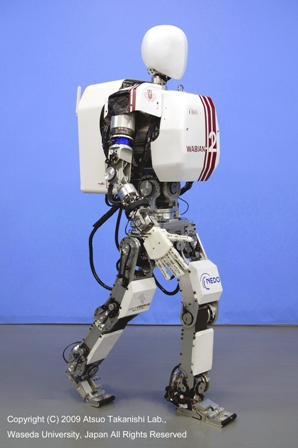
\includegraphics[height=6cm]{robot_wabian.png}
  \caption{WABIAN by Waseda.}
  \label{fig:wabian}
\end{figure}

\subsection{ASIMO by Honda}
ASIMO is a research robot and is not available for commercial sale; it
has, however, been loaned for unique events and used by major companies
as a reception host. As of February 2009, there were over 100 ASIMO
robots in various versions, ultimately aiming to assist individuals who
are disabled, elderly, or ill, and to perform tasks that are dangerous
for humans. The fifth version of ASIMO, released in September 2011,
features enhanced capabilities including the use of all its fingers,
equipped with tactile sensors in the palm and force detectors in each
finger; combined with object-recognition technology, it can pick up a
bottle and unscrew its cap, or hold a paper cup without crushing it. One
of its main innovations is the ability to change direction smoothly
while walking, without interrupting its stride.

\begin{table}[ht]
  \centering
  \caption{Comparison of ASIMO Robot Models.}
  \label{tab:asimo}
  \footnotesize
  \setlength{\tabcolsep}{4pt}
  \renewcommand{\arraystretch}{1.25}
  \begin{tabularx}{\textwidth}{@{}llllXXcc@{}}
    \toprule
    \textbf{Project} & \textbf{Date} & \textbf{Weight} & \textbf{Length}
    & \textbf{Anatomy} & \textbf{Functions} & \textbf{DoF} &
    \textbf{DoF Head} \\
    \midrule
    P-1   & 1993--1997 & 175\,kg & 1.915\,m & Head, Arm, Hand, Leg, Feet, Trunk & Walking & -- & -- \\
    P-2   & --   & 210\,kg & 1.82\,m & -- & Walking, Climbing stairs & 30 & -- \\
    P-3   & --   & 52\,kg  & 1.2\,m  & -- & Speed walking (1.6\,km/h) & 26 & -- \\
    Asimo I   & 2000 & 54\,kg & 1.3\,m & -- & Speed walking (3\,km/h), Object detection, Face recognition & 34 & 3 \\
    Asimo II  & 2005 & 54\,kg & 1.3\,m & -- & Running (6\,km/h), Gripping objects & 34 & 3 \\
    Asimo III & 2011 & 48\,kg & 1.3\,m & -- & Human daily tasks, Collision avoidance, Dynamic path planning & 57 & 3 \\
    \bottomrule
  \end{tabularx}
\end{table}

\begin{figure}[ht]
  \centering
  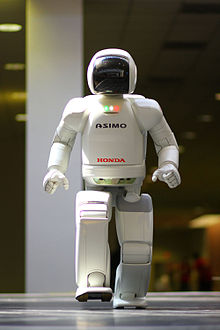
\includegraphics[height=6cm]{robot_asimo.png}
  \caption{ASIMO.}
  \label{fig:asimo}
\end{figure}

\subsection{HRP Humanoid Series by AIST}
The Humanoid Robotics Project (HRP) is an initiative aimed at developing
general domestic-helper robots, funded by Japan's Ministry of Economy,
Trade and Industry (METI) and the New Energy and Industrial Technology
Development Organization (NEDO). The project is led by Kawada Industries
with support from the National Institute of Advanced Industrial Science
and Technology (AIST) and Kawasaki Heavy Industries. The HRP series,
also known as Promet, began with modifications to Honda's P3 robots and
includes features such as a tele-command system. Notably, HRP-2 can
stand up after lying flat, a capability lacking in Honda's ASIMO. The
HRP-4, a bipedal humanoid, stands 150~cm tall and weighs 39~kg.

\begin{table}[ht]
  \centering
  \caption{Comparison of HRP Robot Models.}
  \label{tab:hrp}
  \scriptsize
  \setlength{\tabcolsep}{3pt}
  \renewcommand{\arraystretch}{1.3}
  \begin{tabularx}{\textwidth}{@{}llllXXcXXc@{}}
    \toprule
    \textbf{Project} & \textbf{Date} & \textbf{Weight} & \textbf{Length}
    & \textbf{Anatomy} & \textbf{Functions} & \textbf{DoF} &
    \textbf{DoF Head} & \textbf{DoF Arm} & \textbf{DoF Leg} \\
    \midrule
    HRP-1  & 1998 & 120\,kg & 1.6\,m  & Head, Trunk, Arm, Hand, Leg, Feet & Walking / Hand operations & 30 & 2 & 14: 3 shoulders, 1 elbow, 3 wrist & 12 \\
    HRP-2  & 2003 & 58\,kg  & 1.54\,m & -- & Walking on rug, Standing, Human interaction & 30 & 2 & 12: 3 shoulders, 1 elbow, 2 wrist & 12 \\
    HRP-3  & 2007 & 65\,kg  & 1.6\,m  & -- & Speed walking 2\,km/h & 42 & 2 & 12: 3 shoulders, 1 elbow, 2 wrist & 12 \\
    HRP-4C & 2009 & 43\,kg  & 1.58\,m & -- & Anthropomorphic, Face expressions & 42 & 11: 3 neck, 8 face & 4 & 12 \\
    HRP-4  & 2010 & 39\,kg  & 1.51\,m & -- & Athleticism, Running, Operating tasks & 34 & 2 & 4 & 12 \\
    \bottomrule
  \end{tabularx}
\end{table}

\begin{figure}[ht]
  \centering
  \begin{subfigure}{0.35\textwidth}
    \centering
    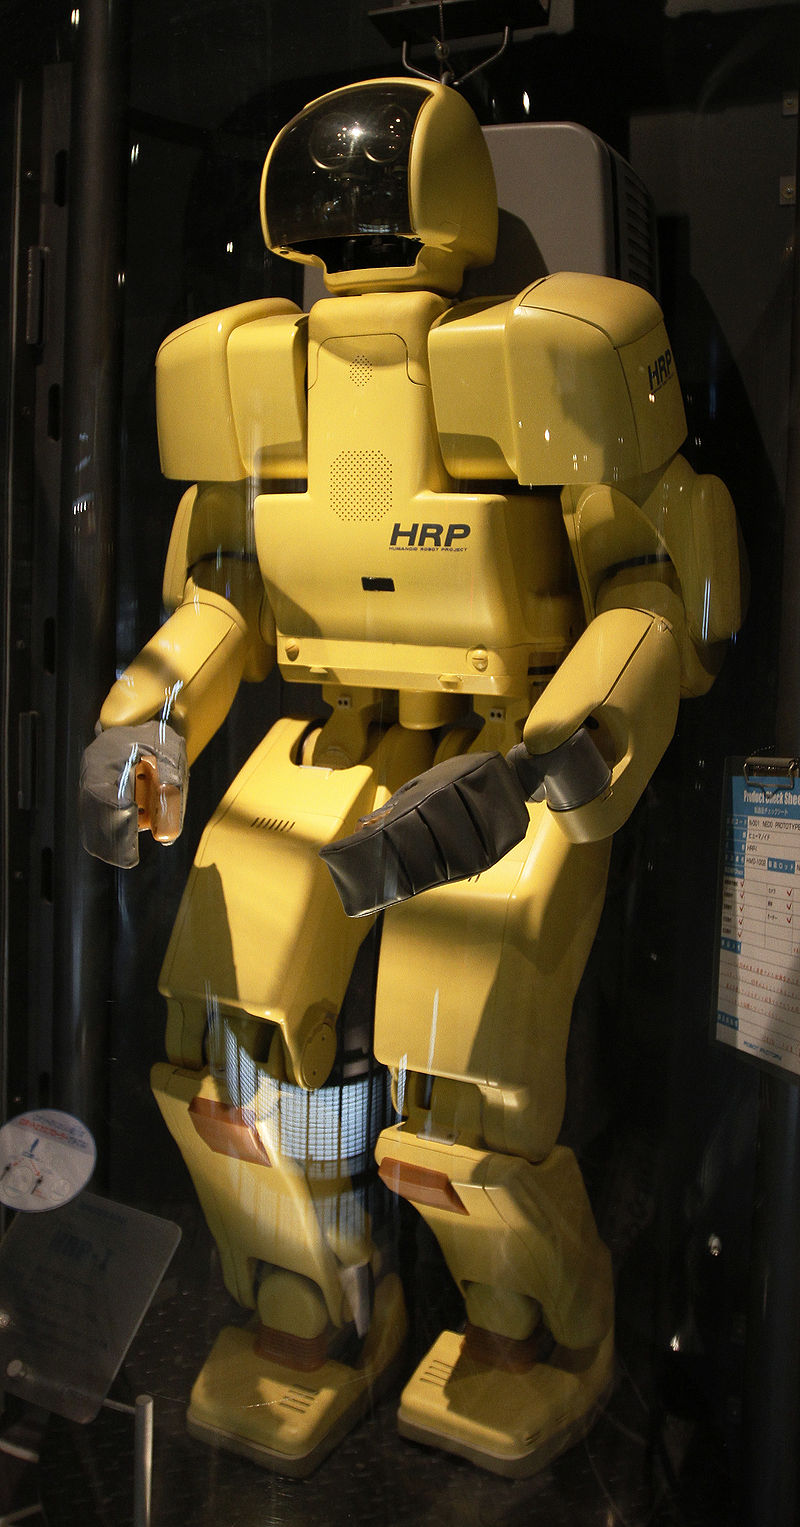
\includegraphics[height=6.5cm]{robot_hrp1.png}
    \caption{HRP-1}
    \label{fig:hrp1}
  \end{subfigure}
  \hspace{1.2cm}
  \begin{subfigure}{0.35\textwidth}
    \centering
    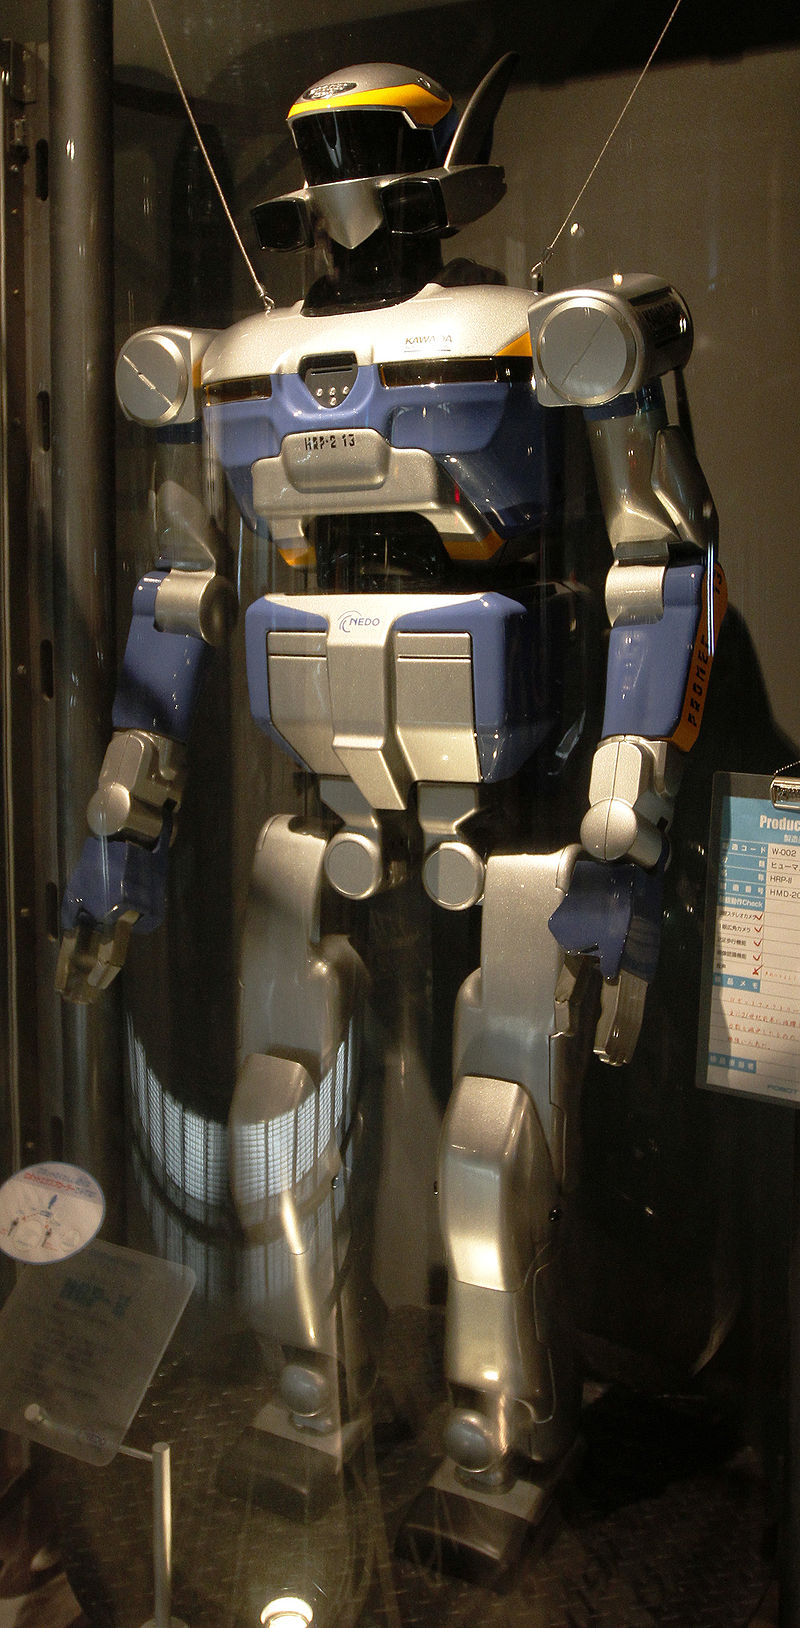
\includegraphics[height=6.5cm]{robot_hrp2.png}
    \caption{HRP-2}
    \label{fig:hrp2}
  \end{subfigure}
  \caption{HRP humanoid robots.}
  \label{fig:hrp}
\end{figure}

\subsection{Positioning of Abbes}
\label{sec:positioning}
The platforms above achieve outstanding performance but rely on custom,
expensive hardware that is out of reach for a student project. Abbes is
positioned instead as a low-cost, fully 3D-printed, 18-DOF humanoid
built around hobby servo-motors and an ESP32 microcontroller. Its
distinguishing contribution is not raw locomotion performance but its
\emph{software}: a modern ROS\,2 control stack with a physics-based
digital twin, and a natural-language command layer driven by a locally
hosted Large Language Model --- a feature uncommon on platforms of this
scale, and the main software-engineering contribution of this work.

\section{Conclusion}
This chapter explored the fundamental principles and obstacles within
bipedal robotics. By examining both the challenges and the
state-of-the-art developments, it identified the critical focal points
for the project. The subsequent chapters delve into the specific
methodologies, design considerations, and practical implementations
required to build the robot. Table~\ref{tab:bipedal} provides a concise
overview of the key features of the robots studied above.

\begin{table}[ht]
  \centering
  \caption{Comparison of Bipedal Robots.}
  \label{tab:bipedal}
  \small
  \renewcommand{\arraystretch}{1.3}
  \begin{tabularx}{\textwidth}{@{}lccX@{}}
    \toprule
    \textbf{Robot} & \textbf{Height (mm)} & \textbf{Number of DoF} &
    \textbf{Capabilities and Features} \\
    \midrule
    WABIAN by Waseda & 1480 & 41 & Human-like gait, stretched knees, heel-contact, toe-off motion \\
    ASIMO by Honda   & Varies & Varies & Bipedal locomotion, object manipulation, human interaction \\
    HRP Series by AIST & Varies & Varies & Anthropomorphic design, various locomotion modes \\
    \bottomrule
  \end{tabularx}
\end{table}

%=====================================================================
%  Chapter 2 — Concepts on Bipedal Walking
%=====================================================================
\chapter{Concepts on Bipedal Walking}
\label{chap:walking}

\section{Introduction}
Bipedal walking, or walking on two legs, is a complex form of locomotion
that involves the coordination of multiple joints to achieve stability,
balance, and forward motion. Understanding its principles is essential
for designing and controlling a humanoid robot. This chapter introduces
the fundamental concepts of bipedal walking: the definition of walking,
the motion planes, the centre of mass, the Zero-Moment-Point, the
support polygon, the stability criteria, the types of walking, and the
gait cycle that together underpin the locomotion work presented later in
this report.

\section{Walking Definition}
Walking can be defined as the action of moving by successive movements
and support of the legs and feet without ever leaving the ground
entirely. This definition does not constrain the number of limbs, so
walking may be bipedal, quadrupedal, and so on; in this work the term
refers to \emph{bipedal} walking, since the objective is to reproduce
human locomotion. Walking is therefore a cyclic phenomenon: each foot
alternately swings through the air and then serves as support, either
alone or together with the other foot. This cyclic nature is formalised
through the notion of gait \emph{cycles} and \emph{phases}, developed in
the following sections.

\section{Motion Planes}
The motion planes describe the movements associated with walking, as
shown in Figure~\ref{fig:planes}. The \textbf{sagittal} plane
corresponds to a side view of the walker, the \textbf{horizontal} plane
to a top view, and the \textbf{frontal} plane to a front view. The
walker moves primarily in the sagittal plane, but movements such as hip
sway, lateral displacement, and pelvic rotation occur in the other two
planes and enhance the fluidity of walking.

\begin{figure}[ht]
  \centering
  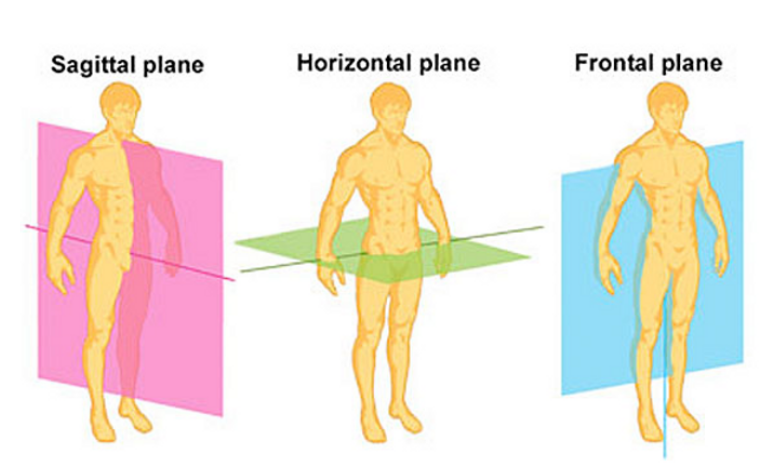
\includegraphics[width=0.75\textwidth]{fig_motion_planes.png}
  \caption{Motion planes: sagittal, horizontal, and frontal.}
  \label{fig:planes}
\end{figure}

\section{Robot Control and Stability}
Bipedal walking relies on several key concepts that ensure stability and
efficiency. These concepts are essential for understanding how to design
and control a bipedal robot.

\subsection{Centre of Mass (CoM)}
The centre of mass (CoM), also known as the centre of gravity, is the
point at which the mass of a body or system of bodies can be considered
to be concentrated. For a rigid body, it is the point at which the body
can be balanced without rotation under the influence of gravity alone.
Mathematically, it is the weighted average of the positions of all the
mass elements of the system. The CoM plays a central role in the study
of the mechanics, dynamics, and stability of a walking robot.

\subsection{Zero-Moment-Point (ZMP)}
The Zero-Moment-Point (ZMP) is a criterion used to analyse the stability
of a bipedal or multi-legged robot during dynamic motion. The ZMP is the
point on the ground where the total moment of the forces acting on the
robot's feet has no horizontal component --- that is, the point where the
ground-reaction forces and the inertial forces acting on the robot's body
balance each other out.

Consider the support foot during the single-support phase
(Figure~\ref{fig:zmp}). The effect of the parts above the support foot
can be replaced by a force $\mathbf{F}$ and a moment $\mathbf{M_A}$ at
the ankle, while the ground reaction $\mathbf{R}$ and moment
$\mathbf{M_S}$ balance the system at the contact point $S$. Because the
ground can only act on the foot through friction and a normal force, the
horizontal moments vanish at this point --- hence the term
\emph{Zero-Moment-Point}. The ZMP is thus the point under the foot where
the ground reaction balances the horizontal moments applied at the
ankle. To maintain dynamic balance, the ZMP must remain inside the
support polygon; if the support area is too small to compensate the
horizontal moment, the robot loses dynamic balance and the ZMP is no
longer defined (a fictitious ZMP may then be computed for analysis).

\begin{figure}[ht]
  \centering
  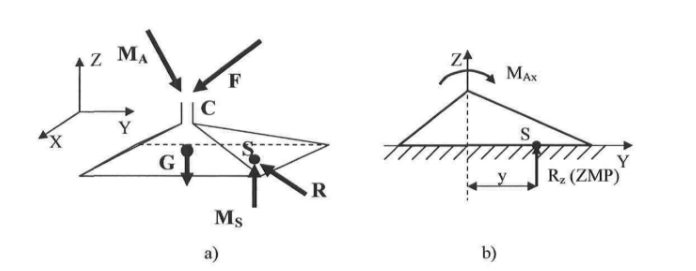
\includegraphics[width=0.85\textwidth]{fig_zmp.png}
  \caption{General case of the ZMP: (a) three-dimensional case at the
           ankle, (b) planar case where the moment $M_{Ax}$ is balanced
           by shifting the point of action of the reaction force $R_z$.}
  \label{fig:zmp}
\end{figure}

\subsection{Support Polygon}
The support polygon is one of the stability criteria for humanoid
walking. It is defined by the outer contour of the points of contact
between the robot's feet and the ground. As illustrated in
Figure~\ref{fig:support}, it takes two forms during the walking cycle:
the \textbf{single-support} polygon, reduced to the contour of a single
foot, and the larger \textbf{double-support} polygon, spanning both feet
when they are simultaneously in contact with the ground.

\begin{figure}[ht]
  \centering
  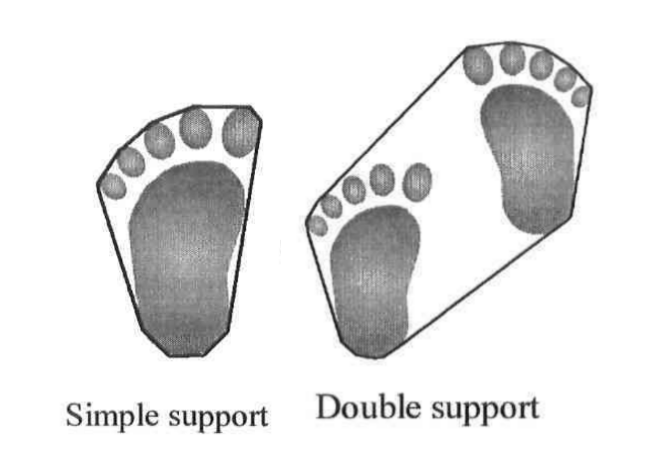
\includegraphics[width=0.55\textwidth]{fig_support_polygon.png}
  \caption{Support polygon in the single- and double-support phases.}
  \label{fig:support}
\end{figure}

\subsection{Stability Criteria}
Two complementary aspects of stability are considered:
\begin{itemize}[itemsep=2pt,topsep=4pt]
  \item \textbf{Posture stability} --- the ability to maintain a stable
        standing position with minimal jerk. Joint positions and the
        centre of gravity are the main variables involved.
  \item \textbf{Gait stability} --- the ability to maintain balance
        during locomotion. The key variables here are step length,
        foothold positions, and ZMP data.
\end{itemize}

\section{Types of Bipedal Walking}
Walking can be categorised into two types:
\begin{itemize}[itemsep=2pt,topsep=4pt]
  \item \textbf{Static walking.} The posture is stable at all times: the
        body weight is always supported by at least one foot, and the
        projection of the CoM on the ground always remains within the
        support polygon.
  \item \textbf{Dynamic walking.} A succession of stable and unstable
        postures. Instability is deliberately created forward when the
        projection of the CoM moves outside the support polygon. Dynamic
        walking is the natural human gait; the resulting instability is
        corrected by the next step.
\end{itemize}

\section{Robot Gait Generation}

\subsection{Walking-Cycle Components}
Ignoring the very first and very last steps to and from a standing
posture, the walking cycle is composed of two alternating phases:
\begin{description}[itemsep=2pt,topsep=4pt]
  \item[Double-Support Phase (DSP)] The robot is in contact with the
        floor through both legs. This phase lets the robot shift its ZMP
        into a favourable position for the next step without losing
        balance; it is therefore called the \emph{stabilisation} phase.
  \item[Single-Support Phase (SSP)] Also known as the swing phase, the
        robot is in contact with the floor through a single leg. The leg
        in contact is the \emph{support} leg and the other is the
        \emph{swinging} leg.
\end{description}

\subsection{Walking-Cycle Phases}
Within these components, the cycle progresses through the following
phases:
\begin{itemize}[itemsep=2pt,topsep=4pt]
  \item \textbf{Impact / contact phase (DSP)} --- the heel of the front
        foot comes into contact with the floor.
  \item \textbf{Lift-off / swing phase (SSP)} --- during the transition
        from double to single support, the swinging foot is lifted off
        the ground; the robot transfers its weight onto the support foot
        and starts swinging the rear leg forward.
  \item \textbf{Catch phase (DSP)} --- the swinging foot comes back into
        contact with the floor, returning the robot to double support.
\end{itemize}
The roles of the two legs are then swapped and the cycle repeats.

\subsection{Gait Engine}
The gait engine, also referred to as the walking-pattern generator, is
the software component responsible for producing a sequence of feasible
joint positions that reproduce a walking motion. It accounts for the
robot's physical limitations, its preferred walking speed, and the
desired gait style to compute the best sequence of joint angles and body
motions for stable and efficient walking. Gait engines fall into two
main families:
\begin{itemize}[itemsep=2pt,topsep=4pt]
  \item \textbf{ZMP-based approach} --- requires comprehensive knowledge
        of the robot's parameters and uses the ZMP as a feedback signal
        to adjust joint angles and torques.
  \item \textbf{Inverted-pendulum approach} --- operates with limited
        knowledge of the robot model and uses a closed-loop feedback
        based on the inverted-pendulum abstraction.
\end{itemize}
The gait generator developed in this work follows the ZMP-based approach
and is detailed in Chapter~\ref{chap:kinematics}.

\section{Walking Primitive}
A walking primitive is a fundamental building block that generates the
motion of a robot's gait. It defines characteristics such as step
length, step height, and step frequency, taking into account the robot's
physical constraints, its stability requirements, and the desired
locomotion behaviour.

\section{Conclusion}
This chapter introduced the fundamental concepts of bipedal walking,
providing the vocabulary and the stability criteria --- centre of mass,
Zero-Moment-Point, and support polygon --- that govern stable, human-like
locomotion, together with the structure of the gait cycle. These
concepts form the theoretical foundation for the hardware, firmware, and
control chapters that follow. The next chapter presents the hardware and
mechatronic design of the Abbes robot.

%=====================================================================
%  Chapter 3 — Hardware and Mechatronic Design
%=====================================================================
\chapter{Hardware and Mechatronic Design}
\label{chap:hardware}

\section{Introduction}
Designing a bipedal robot is a multidisciplinary task that combines
principles from mechanical engineering, electronics, and computer
science. This chapter presents the physical foundation of the
\textbf{Abbes} robot: the mechanical design derived from human
proportions, the selection of actuators and sensors, the power supply,
and the electronic architecture built around an ESP32 microcontroller.
Together these subsystems form the platform on which the firmware and
control software of the following chapters run.

\section{Mechanical Design}
The mechanical design is inspired by the anatomical structure of the
human body. As the review of existing humanoids in
Chapter~\ref{chap:presentation} showed, the construction of humanoid
robots is rooted in mimicking human morphology.

\subsection{Anthropometric Model}
The anthropometric model expresses the robot's dimensions as a function
of human-body proportions, so that its segments and movements stay as
close to human anatomy as possible. Anthropometry --- from the Greek
\emph{anthropos} (human) and \emph{metron} (measure) --- is the study
and measurement of the physical dimensions of the human body. This work
relies on \emph{static} anthropometric measurements, whose implementation
is simpler, using the normalised segmental proportions established by
Winter. Figure~\ref{fig:anthropometric} gives the length of each limb
relative to the total height $H$ of the individual.

\begin{figure}[ht]
  \centering
  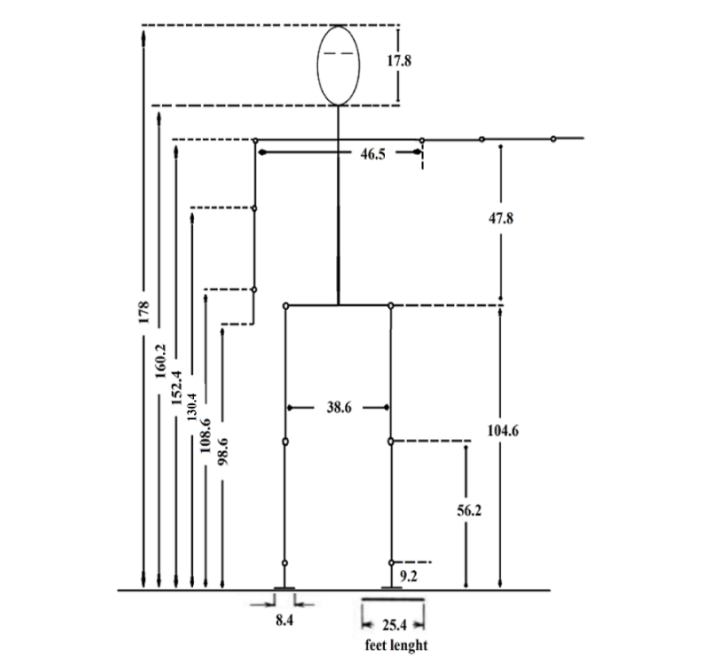
\includegraphics[width=0.6\textwidth]{fig_anthropometric.png}
  \caption{Anthropometric model: segment lengths as a proportion of
           total height $H$ (Winter's model).}
  \label{fig:anthropometric}
\end{figure}

\subsection{Mechanical Articulated Structure}
The articulated structure is the set of interconnected joints and links
that lets the robot reproduce human-like movements. The number of
degrees of freedom (DOF) must be large enough for agility and balance,
yet kept minimal to simplify the model. For a leg, two DOF (at the hip
and ankle) enable pendulum-like motion in the sagittal plane, and two
more provide lateral motion in the frontal plane; a fifth DOF at the knee
is required to clear the foot during the swing phase. This leads to five
DOF per leg. Each arm uses three DOF, and the head two, as detailed in
the next section. Figure~\ref{fig:morphology} shows the resulting joint
arrangement.

\begin{figure}[ht]
  \centering
  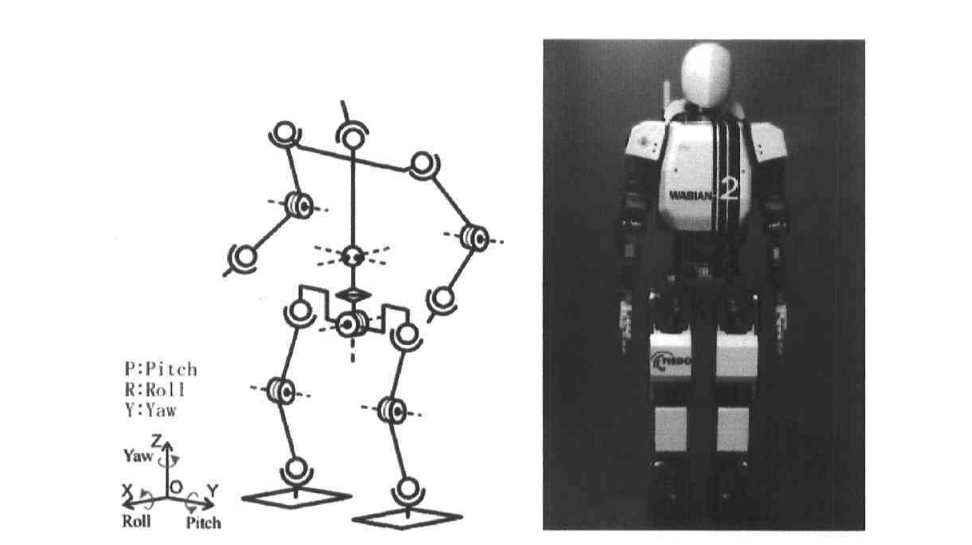
\includegraphics[width=0.7\textwidth]{fig_morphology.png}
  \caption{Robot morphology: joint arrangement and reference frame
           (P: pitch, R: roll, Y: yaw).}
  \label{fig:morphology}
\end{figure}

\subsection{Final Design: Joint Limits and Resting Positions}
The final design is an 18-DOF humanoid with the following distribution:
\begin{itemize}[itemsep=2pt,topsep=4pt]
  \item \textbf{Each leg --- 5 DOF:} 2 at the hip (pitch and roll),
        1 at the knee (pitch), and 2 at the ankle (pitch and roll).
  \item \textbf{Each arm --- 3 DOF:} 2 at the shoulder (pitch and roll)
        and 1 at the elbow (roll).
  \item \textbf{Head --- 2 DOF:} head yaw and camera pitch.
\end{itemize}

Table~\ref{tab:joints} summarises the complete joint structure. The
angle range and resting position of each joint are expressed in degrees
of servo travel; these exact values are the single source of truth used
by the firmware (the limits are enforced before any command reaches a
servo, see Chapter~\ref{chap:firmware}). The joints are listed in the
firmware's index order, which groups the right-side joints and the head
on the first PWM board and the left-side joints on the second.

\begin{table}[ht]
  \centering
  \caption{Robot joint structure: axes, angular limits and resting
           positions (servo degrees).}
  \label{tab:joints}
  \small
  \setlength{\tabcolsep}{6pt}
  \renewcommand{\arraystretch}{1.12}
  \begin{tabular}{@{}clccccc@{}}
    \toprule
    \textbf{\#} & \textbf{Joint name} & \textbf{Axis} &
    \textbf{Min ($^\circ$)} & \textbf{Max ($^\circ$)} &
    \textbf{Rest ($^\circ$)} \\
    \midrule
    1  & r\_shoulder\_pitch & pitch & 0  & 180 & 90  \\
    2  & r\_shoulder\_roll  & roll  & 0  & 180 & 90  \\
    3  & r\_elbow\_roll     & roll  & 0  & 180 & 90  \\
    4  & head\_yaw          & yaw   & 0  & 180 & 90  \\
    5  & camera\_pitch      & pitch & 0  & 180 & 90  \\
    6  & r\_hip\_roll       & roll  & 0  & 170 & 50  \\
    7  & r\_hip\_pitch      & pitch & 0  & 170 & 80  \\
    8  & r\_knee\_pitch     & pitch & 0  & 170 & 100 \\
    9  & r\_ankle\_pitch    & pitch & 10 & 180 & 100 \\
    10 & r\_ankle\_roll     & roll  & 20 & 150 & 90  \\
    11 & l\_shoulder\_pitch & pitch & 0  & 180 & 90  \\
    12 & l\_shoulder\_roll  & roll  & 0  & 180 & 90  \\
    13 & l\_elbow\_roll     & roll  & 0  & 180 & 90  \\
    14 & l\_hip\_roll       & roll  & 0  & 170 & 50  \\
    15 & l\_hip\_pitch      & pitch & 0  & 170 & 80  \\
    16 & l\_knee\_pitch     & pitch & 0  & 170 & 70  \\
    17 & l\_ankle\_pitch    & pitch & 10 & 180 & 90  \\
    18 & l\_ankle\_roll     & roll  & 20 & 150 & 90  \\
    \bottomrule
  \end{tabular}
\end{table}

The mechanical parts are designed in CAD (Figure~\ref{fig:cad}) and
manufactured by 3D printing; the assembled robot is shown in
Figure~\ref{fig:realrobot}.

\begin{figure}[ht]
  \centering
  \begin{subfigure}{0.40\textwidth}
    \centering
    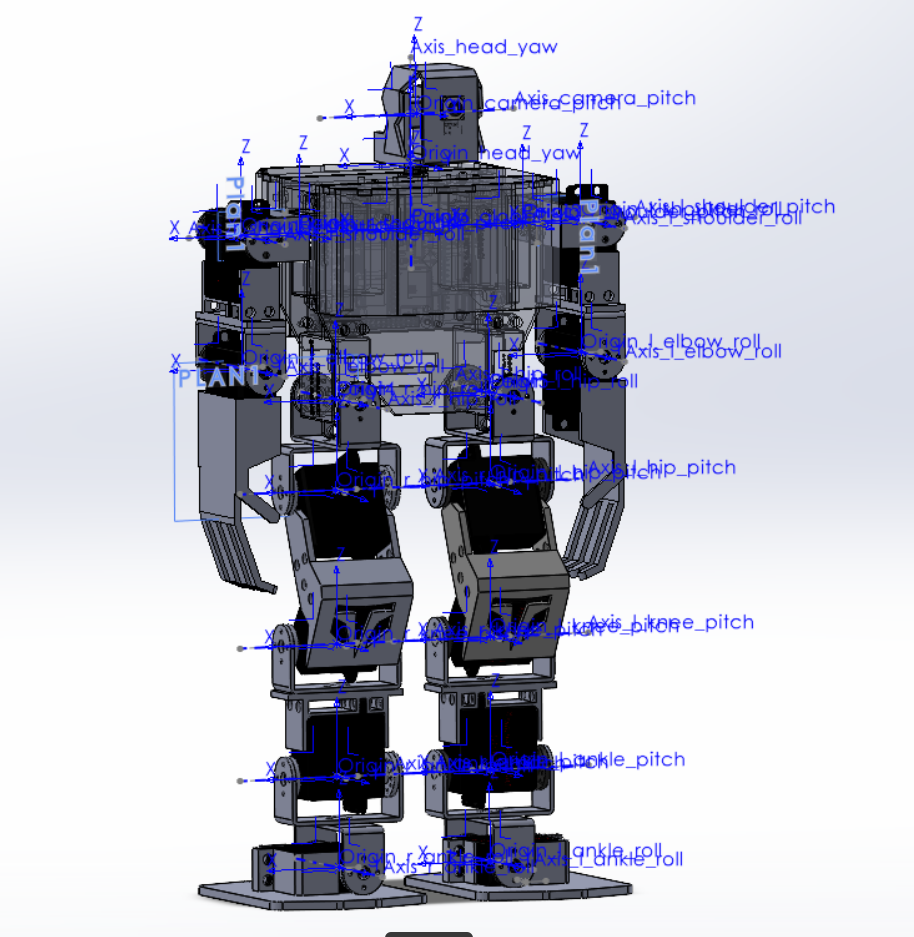
\includegraphics[height=6.5cm]{fig_cad_design.png}
    \caption{CAD model}
    \label{fig:cad}
  \end{subfigure}
  \hspace{0.8cm}
  \begin{subfigure}{0.40\textwidth}
    \centering
    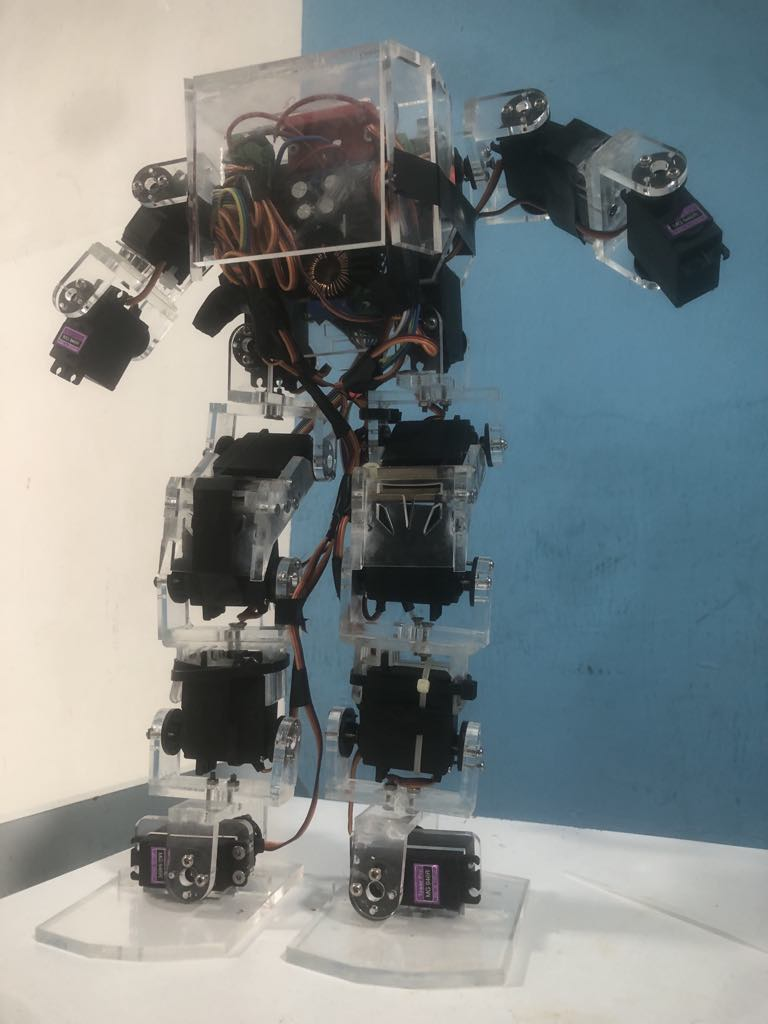
\includegraphics[height=6.5cm]{fig_real_robot.png}
    \caption{Assembled robot}
    \label{fig:realrobot}
  \end{subfigure}
  \caption{Mechanical design of Abbes: (a) CAD model and (b) the
           3D-printed, assembled robot.}
  \label{fig:mechanical}
\end{figure}

\section{Hardware Components}

\subsection{Actuators}
Selecting actuators involves several criteria: high torque and precision
for accurate motion, efficient current consumption, a size and weight
compatible with the structure, durability, and cost. Table~\ref{tab:act}
compares the candidates considered. The \textbf{MG996R} servo was
selected: it offers a sufficient torque-to-cost ratio for a child-sized,
3D-printed platform, and it is directly compatible with standard PWM
control. The robot uses eighteen such servos, one per joint.

\begin{table}[ht]
  \centering
  \caption{Actuator specifications.}
  \label{tab:act}
  \small
  \renewcommand{\arraystretch}{1.2}
  \begin{tabularx}{\textwidth}{@{}lccccc@{}}
    \toprule
    \textbf{Actuator} & \textbf{Model} & \textbf{Price (\euro)} &
    \textbf{Torque (kg$\cdot$cm)} & \textbf{Position sensor} &
    \textbf{Current (A)} \\
    \midrule
    Servo      & MG996R  & 20    & 10        & --          & 1   \\
    Dynamixel  & MX-28   & 312   & 31.6      & Contactless & 1.7 \\
    Servo      & HS-645MG& 38.40 & 107 / 133 & --          & 2.5 \\
    \bottomrule
  \end{tabularx}
\end{table}

\subsection{Sensors}
The robot's primary sensor is the \textbf{MPU6050}, which combines a
three-axis gyroscope and a three-axis accelerometer in a single
low-cost, I\textsuperscript{2}C-compatible package
(Table~\ref{tab:sensor}). It provides the angular-velocity and
acceleration data needed to estimate the robot's orientation and to
maintain balance during motion. Its digital interface simplifies
integration with the microcontroller.

\begin{table}[ht]
  \centering
  \caption{Sensor description.}
  \label{tab:sensor}
  \small
  \renewcommand{\arraystretch}{1.2}
  \begin{tabularx}{0.7\textwidth}{@{}lX@{}}
    \toprule
    \textbf{Sensor} & \textbf{Description} \\
    \midrule
    MPU6050 & Combines a three-axis gyroscope and a three-axis
              accelerometer (raw I\textsuperscript{2}C). \\
    \bottomrule
  \end{tabularx}
\end{table}

\subsection{Power Supply}
The power supply must deliver the voltage and current required by all
components within budget constraints. The robot is \emph{currently
powered from an off-board source}; a battery-powered version is planned
as future work. Table~\ref{tab:battery} lists the battery options
selected for that version: a high-capacity LiPo pack is preferred for its
current rating, at a higher cost than a basic lithium cell.

\begin{table}[ht]
  \centering
  \caption{Battery specifications.}
  \label{tab:battery}
  \small
  \renewcommand{\arraystretch}{1.2}
  \begin{tabular}{@{}lcc@{}}
    \toprule
    \textbf{Battery} & \textbf{Current rating (mAh)} & \textbf{Cost} \\
    \midrule
    LiPo    & 5000 & High \\
    Lithium & 1000 & Low  \\
    \bottomrule
  \end{tabular}
\end{table}

\subsection{DC/DC Regulator}
A DC/DC converter adapts the battery voltage to the levels required by
the servos and the electronics. Table~\ref{tab:regulator} compares the
regulators considered, trading current rating against cost.

\begin{table}[ht]
  \centering
  \caption{Regulator specifications.}
  \label{tab:regulator}
  \small
  \renewcommand{\arraystretch}{1.2}
  \begin{tabular}{@{}lcc@{}}
    \toprule
    \textbf{Regulator} & \textbf{Current rating (A)} & \textbf{Cost (\euro)} \\
    \midrule
    XL6009 & 3.0 & 14 \\
    XL4016 & 9.0 & 30 \\
    LM2596 & 1.5 & 8  \\
    \bottomrule
  \end{tabular}
\end{table}

\section{Electronic Architecture}
\label{sec:hw-arch}
The robot's electronics are organised into a \textbf{control section} and
a \textbf{power section}.

The control section is built around an \textbf{ESP32 microcontroller},
which runs the real-time control loop directly on the robot and joins the
ROS\,2 graph as a \emph{micro-ROS} node over WiFi/UDP. The ESP32 drives
the eighteen servos through \textbf{two PCA9685} 16-channel PWM driver
boards on the I\textsuperscript{2}C bus (at addresses 0x40 and 0x41): the
first board carries the right-side and head joints, the second the
left-side joints. The same I\textsuperscript{2}C bus connects the
\textbf{MPU6050} IMU. On the host (laptop) side, a micro-ROS \emph{agent}
bridges the ESP32 into ROS\,2, so that the inertial data published by the
node and the joint commands it receives are available as ordinary ROS\,2
topics. This architecture replaces the more common pairing of a
single-board computer with a separate servo controller by a single,
low-cost microcontroller that communicates wirelessly. The power section
supplies the servos and electronics through the battery and DC/DC
regulator described above. Figure~\ref{fig:hwarch} summarises the
architecture.

\begin{figure}[ht]
  \centering
  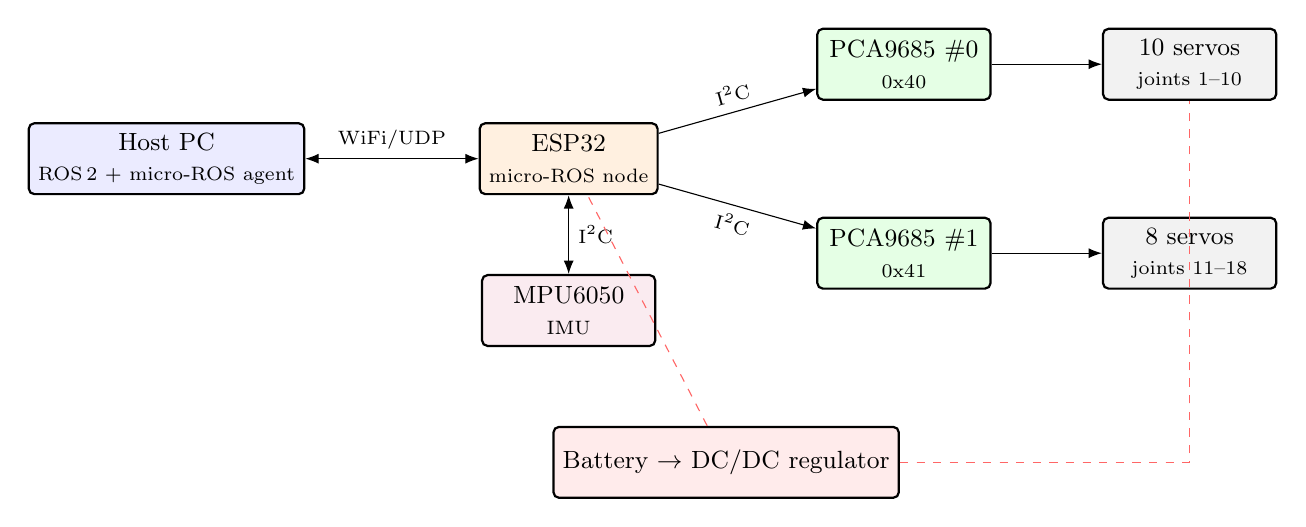
\begin{tikzpicture}[
      font=\small,
      box/.style={draw, rounded corners=2pt, align=center,
                  minimum height=9mm, minimum width=22mm, thick},
      host/.style={box, fill=blue!8},
      mcu/.style={box, fill=orange!12},
      drv/.style={box, fill=green!10},
      sen/.style={box, fill=purple!8},
      pwr/.style={box, fill=red!8},
      >=Latex
    ]
    \node[host] (host) {Host PC\\\scriptsize ROS\,2 + micro-ROS agent};
    \node[mcu, right=22mm of host] (esp) {ESP32\\\scriptsize micro-ROS node};
    \node[drv, right=20mm of esp, yshift=12mm] (pca0) {PCA9685 \#0\\\scriptsize 0x40};
    \node[drv, right=20mm of esp, yshift=-12mm] (pca1) {PCA9685 \#1\\\scriptsize 0x41};
    \node[sen, below=10mm of esp] (imu) {MPU6050\\\scriptsize IMU};
    \node[box, right=14mm of pca0, fill=gray!10] (s0) {10 servos\\\scriptsize joints 1--10};
    \node[box, right=14mm of pca1, fill=gray!10] (s1) {8 servos\\\scriptsize joints 11--18};
    \node[pwr, below=10mm of imu, xshift=20mm] (pwr) {Battery $\rightarrow$ DC/DC regulator};

    \draw[<->] (host) -- node[above,font=\scriptsize]{WiFi/UDP} (esp);
    \draw[->] (esp) -- node[above,sloped,font=\scriptsize]{I\textsuperscript{2}C} (pca0);
    \draw[->] (esp) -- node[below,sloped,font=\scriptsize]{I\textsuperscript{2}C} (pca1);
    \draw[<->] (esp) -- node[right,font=\scriptsize]{I\textsuperscript{2}C} (imu);
    \draw[->] (pca0) -- (s0);
    \draw[->] (pca1) -- (s1);
    \draw[-, dashed, red!60] (pwr) -- (esp);
    \draw[-, dashed, red!60] (pwr) -| (s0);
    \draw[-, dashed, red!60] (pwr) -| (s1);
  \end{tikzpicture}
  \caption{Electronic architecture of Abbes: the ESP32 micro-ROS node
           drives 18 servos through two PCA9685 boards and reads the
           MPU6050, communicating with the ROS\,2 host over WiFi. Dashed
           red lines indicate power distribution.}
  \label{fig:hwarch}
\end{figure}

\section{Conclusion}
This chapter presented the hardware foundation of Abbes. The mechanical
structure was derived from anthropometric data to obtain a human-like,
18-DOF morphology, and its joint limits were defined
(Table~\ref{tab:joints}). The components were selected to balance
performance, cost, and efficiency: MG996R servos, an MPU6050 IMU, and a
battery/regulator pair for the powered version. The electronic
architecture is built around an ESP32 that drives the servos through two
PCA9685 boards and joins ROS\,2 as a micro-ROS node. The next chapter
details the embedded firmware that runs on this ESP32.

%=====================================================================
%  Chapter 4 — Embedded Firmware: the ESP32 micro-ROS Node
%=====================================================================
\chapter{Embedded Firmware: the On-Board Controller}
\label{chap:firmware}

\section{Introduction}
The firmware is the lowest software layer of the robot: it runs directly
on the microcontroller introduced in Chapter~\ref{chap:hardware} and
turns the electronics into an active component of the robot's software
system. Its responsibilities are concrete: receive the eighteen target
joint angles, drive the actuated servos smoothly through the PCA9685
board, read the MPU6050 inertial sensor, and make all of this available to the
rest of the system. This chapter first justifies the choice of the ESP32,
then explains how the firmware is organised, how it handles the actuators
and sensors over the I\textsuperscript{2}C bus, and finally how it joins
the ROS\,2 world through \emph{micro-ROS} --- the bridge that leads
naturally into the next chapter.

\section{Choice of the ESP32}
\label{sec:choice-esp}
The on-board controller has a demanding but bounded role: it must update
eighteen servos and sample an inertial sensor at a steady rate, while
exchanging data with the host computer. Selecting a microcontroller for
this task involves balancing computing power, connectivity, and cost.

The \textbf{ESP32} was chosen because it meets all of these constraints
at once. It is a low-cost, dual-core processor running at 240~MHz with
enough memory to host a lightweight ROS\,2 client, which is far beyond
the reach of an 8-bit board such as a basic Arduino. Crucially, it
integrates \textbf{WiFi}, allowing the robot to communicate with the host
wirelessly and to operate untethered. It natively supports the
\textbf{I\textsuperscript{2}C} bus required by both the PCA9685 PWM
drivers and the MPU6050 sensor, and it runs a real-time operating system
(FreeRTOS) whose two cores can separate time-critical communication from
supervision. Finally, it is well supported by the embedded ROS\,2
tooling used in this project. Compared with a single-board computer such
as a Raspberry Pi, the ESP32 is cheaper, lighter, and consumes far less
power --- and the modest computation performed on board does not require
a full operating system, making the single-board computer unnecessary
for this layer.

\section{Firmware Architecture}
\label{sec:fw-arch}
The firmware is written in C++ on the Arduino/PlatformIO framework and is
deliberately split into focused modules rather than a single monolithic
program: one module manages the servos, one is a self-contained driver
for the IMU, and one handles the communication with the host. A separate
file holds the joint map (Table~\ref{tab:joints}) and all hardware
constants, so that no hardware-specific value is hidden in the logic.

The architecture takes advantage of the ESP32's two cores. All
communication --- the wireless link, the connection lifecycle, and the
dispatching of incoming and outgoing messages --- runs in a dedicated
real-time task pinned to \textbf{core~1}. \textbf{Core~0} is left to the
main program, which only supervises the system and is reserved for future
watchdog and safety logic. Separating communication from supervision in
this way ensures that activity on the network cannot stall the safety
logic, and vice versa.

Functionally, the firmware implements two continuous data paths, shown in
Figure~\ref{fig:fwflow}. On the \emph{command path}, target joint angles
arriving from the host are stored, and a periodic 100~Hz routine drives
the servos toward those targets through the PWM boards. On the
\emph{sensing path}, the inertial sensor is sampled and a periodic 50~Hz
routine sends the measurements back to the host. Both periodic routines
are driven by the microcontroller's own clock, so the joint-control rate
remains regular even when network traffic is not. On start-up, the same
servo mechanism first brings all joints smoothly to their resting
position before any command is accepted.

\begin{figure}[ht]
  \centering
  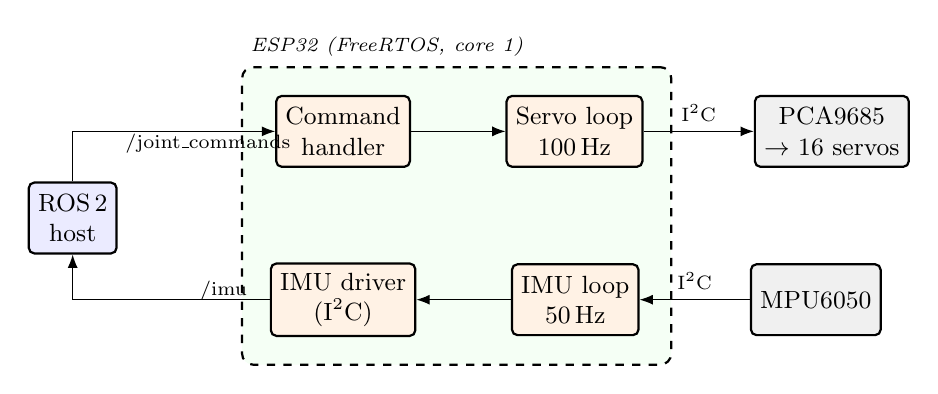
\begin{tikzpicture}[
      font=\small, >=Latex,
      mod/.style={draw, rounded corners=2pt, align=center, thick,
                  minimum height=9mm, fill=orange!10},
      hw/.style={draw, rounded corners=2pt, align=center, thick,
                 minimum height=9mm, fill=gray!12},
      ext/.style={draw, rounded corners=2pt, align=center, thick,
                  minimum height=9mm, fill=blue!8},
    ]
    \node[ext] (host) {ROS\,2\\host};
    \node[mod, right=20mm of host, yshift=11mm] (sub) {Command\\handler};
    \node[mod, right=12mm of sub] (servo) {Servo loop\\100\,Hz};
    \node[mod, below=12mm of sub] (imudrv) {IMU driver\\(I\textsuperscript{2}C)};
    \node[mod, right=12mm of imudrv] (imutim) {IMU loop\\50\,Hz};
    \node[hw, right=14mm of servo] (pca) {PCA9685\\$\rightarrow$ 16 servos};
    \node[hw, right=14mm of imutim] (imu) {MPU6050};

    \begin{scope}[on background layer]
      \node[draw, dashed, thick, rounded corners, fill=green!4,
            fit=(sub)(servo)(imudrv)(imutim), inner sep=10pt] (esp) {};
      \node[anchor=south west, font=\scriptsize\itshape]
            at (esp.north west) {ESP32 (FreeRTOS, core 1)};
    \end{scope}

    \draw[->] (host.north) |- (sub.west) node[midway,above,font=\scriptsize]{};
    \draw[->] (sub) -- (servo);
    \draw[->] (servo) -- node[above,font=\scriptsize]{I\textsuperscript{2}C} (pca);
    \draw[->] (imu) -- node[above,font=\scriptsize]{I\textsuperscript{2}C} (imutim);
    \draw[->] (imutim) -- (imudrv);
    \draw[->] (imudrv.west) -| (host.south);
    \node[font=\scriptsize] at ($(host)!0.5!(sub)+(0,4mm)$) {/joint\_commands};
    \node[font=\scriptsize] at ($(host)!0.5!(imudrv)+(2mm,-4mm)$) {/imu};
  \end{tikzpicture}
  \caption{Firmware data paths: the command path (top) drives the servos
           at 100~Hz, the sensing path (bottom) publishes the IMU at
           50~Hz. Both periodic loops run on the microcontroller's clock.}
  \label{fig:fwflow}
\end{figure}

The on-board electronics that implement this architecture are shown in
Figure~\ref{fig:onboard}: the ESP32 controller with its servo-driver
board and wiring harness, and the DC-DC regulators that power the
actuators.

\begin{figure}[ht]
  \centering
  \begin{subfigure}{0.52\textwidth}
    \centering
    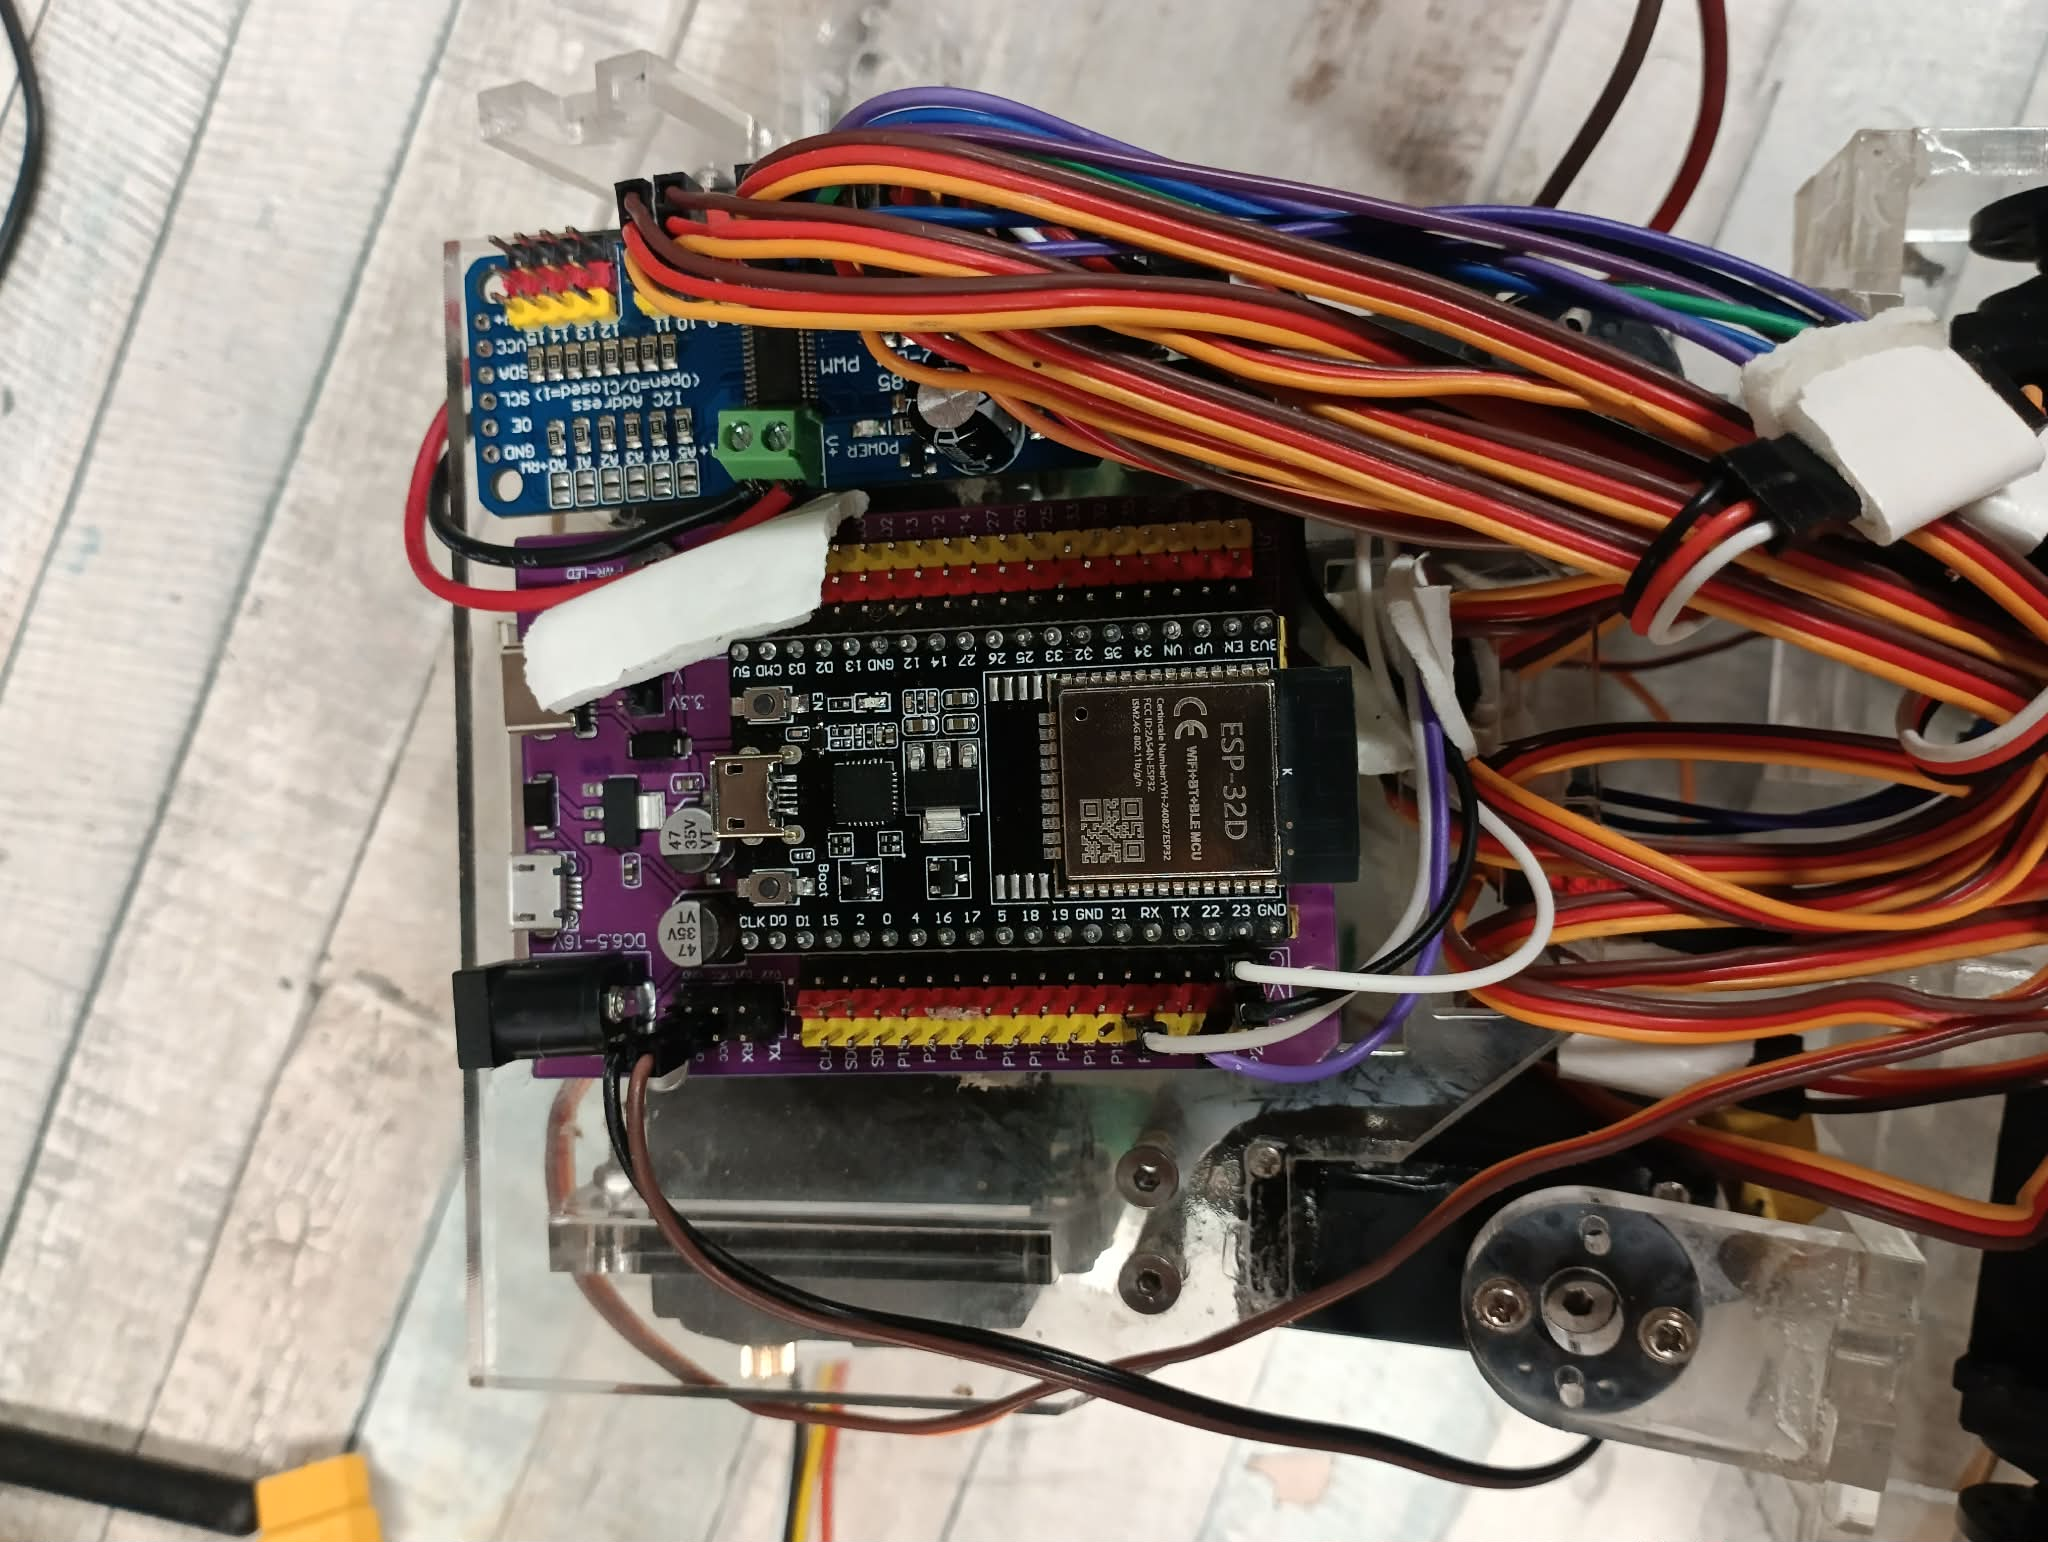
\includegraphics[height=5.5cm]{bor1.jpeg}
    \caption{ESP32 controller and PWM servo driver}
    \label{fig:onboard-esp}
  \end{subfigure}
  \hfill
  \begin{subfigure}{0.40\textwidth}
    \centering
    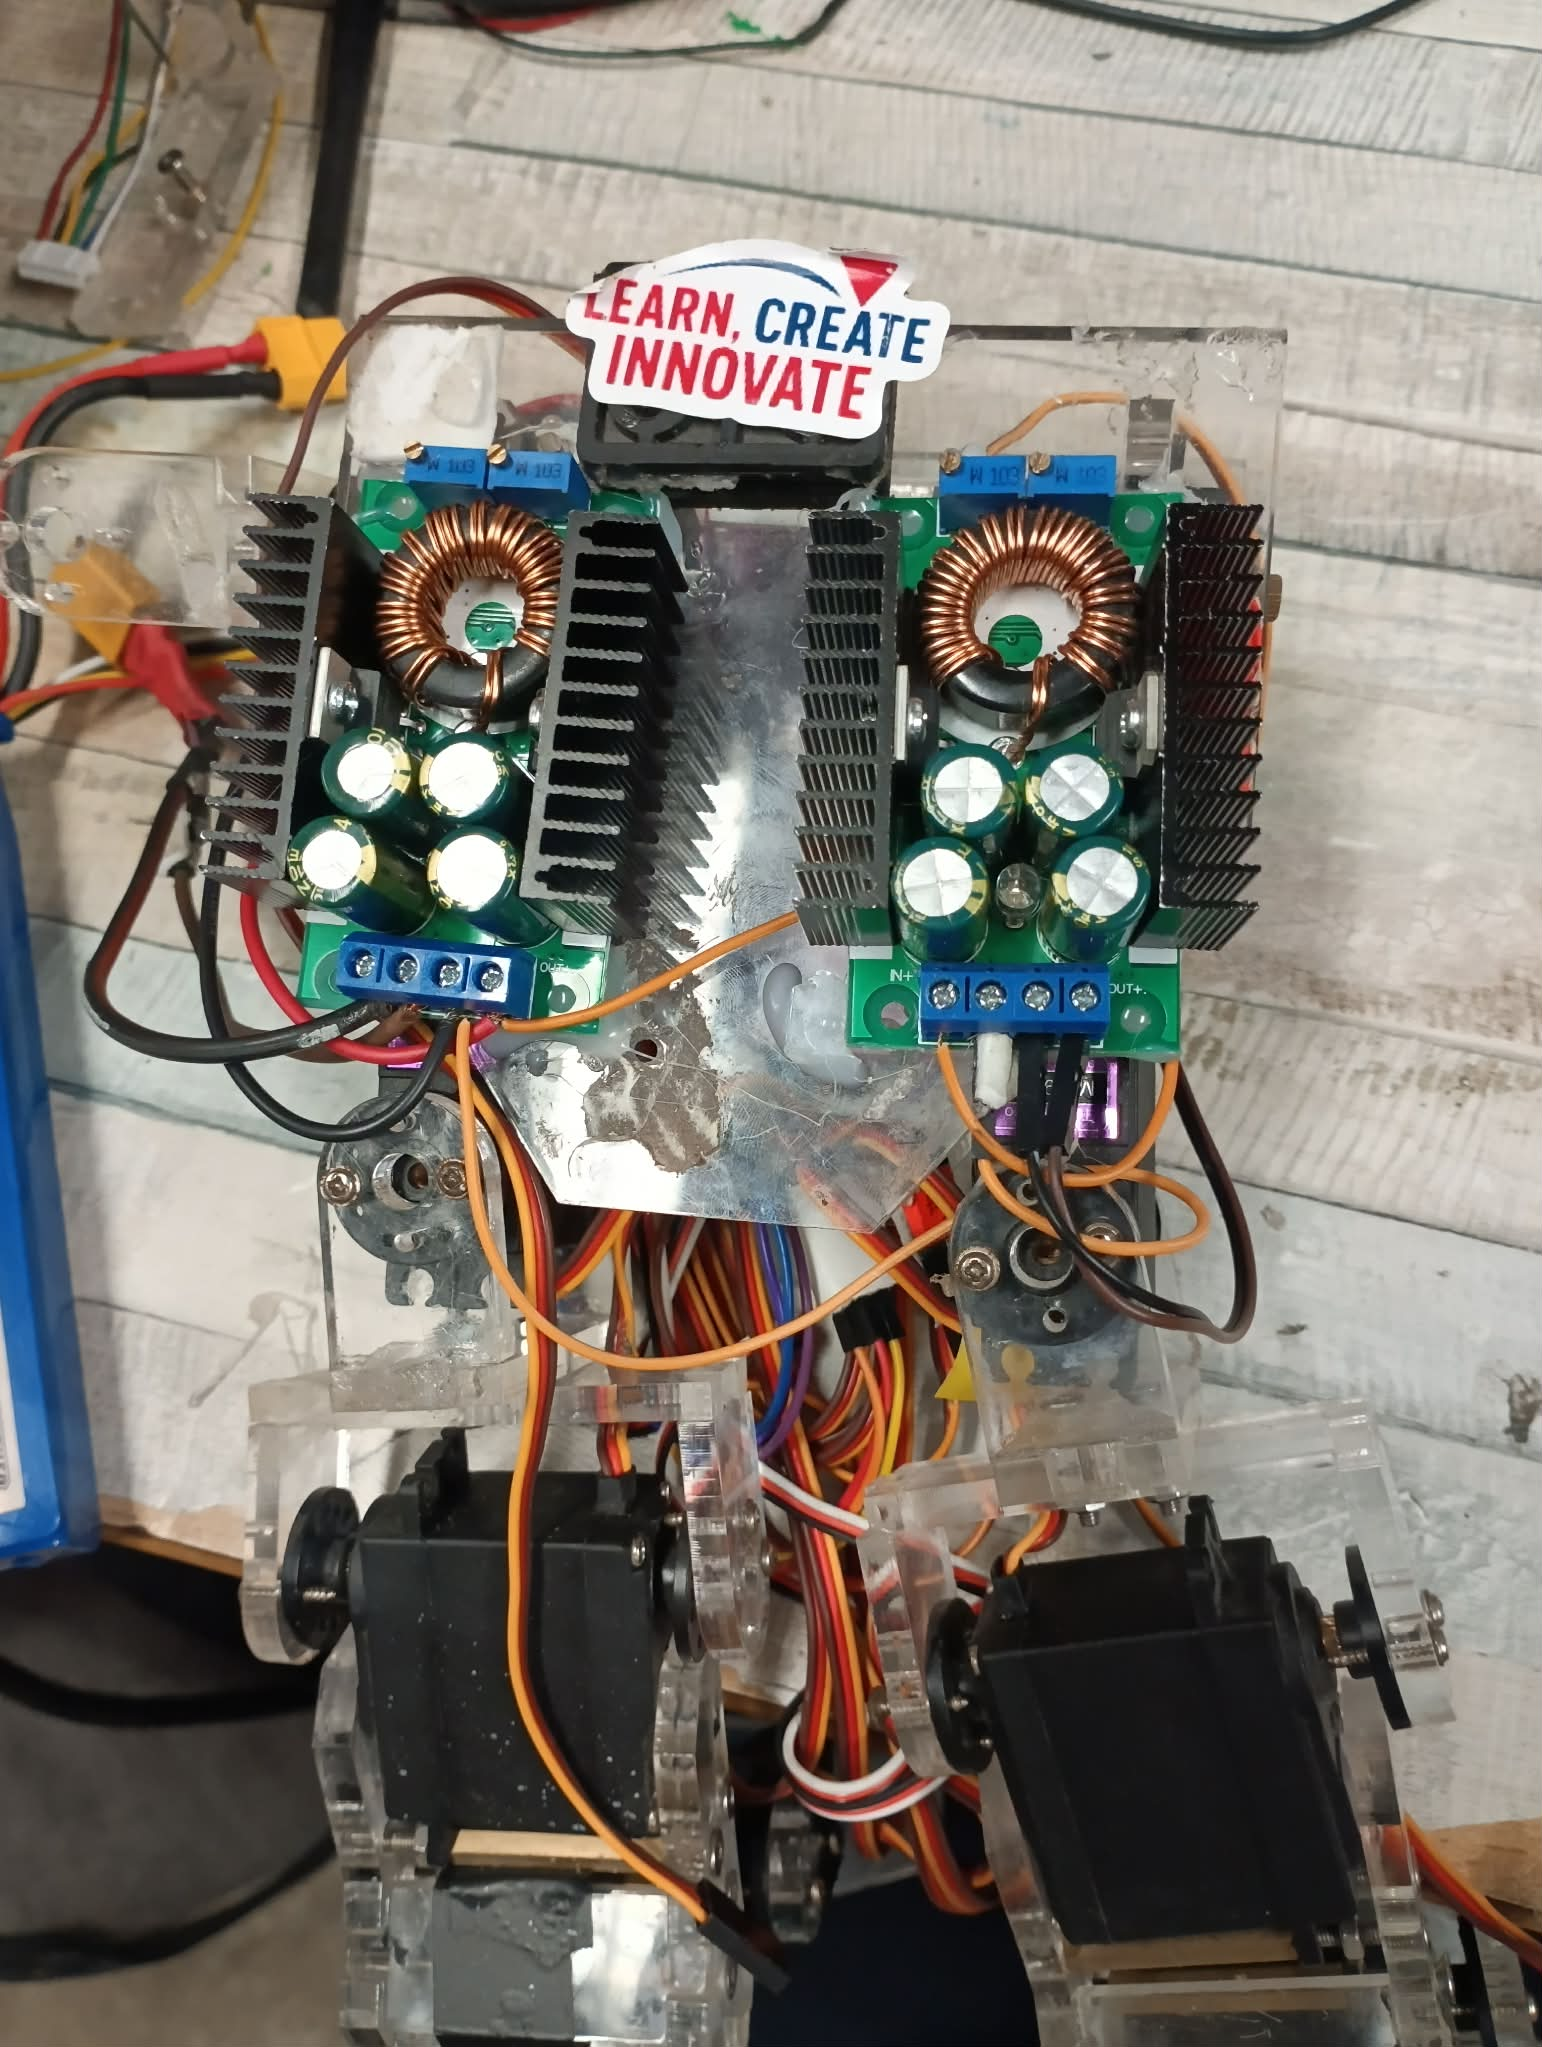
\includegraphics[height=5.5cm]{bor2.jpeg}
    \caption{DC-DC power regulators}
    \label{fig:onboard-pwr}
  \end{subfigure}
  \caption{On-board electronics of Abbes: (a) the ESP32 with the PCA9685
           servo driver and the servo wiring harness, and (b) the DC-DC
           regulators supplying the actuators.}
  \label{fig:onboard}
\end{figure}

\section{Actuators and Sensors over I\texorpdfstring{\textsuperscript{2}}{2}C}
\label{sec:fw-io}
The PWM driver boards and the inertial sensor all share a single
\textbf{I\textsuperscript{2}C} bus, a two-wire serial bus on which each
device has its own address. This is what allows the peripherals --- the
PCA9685 PWM driver (at address 0x40) and the MPU6050 --- to be controlled
through only two microcontroller pins.

\paragraph{Actuators.}
A joint angle cannot be sent to a servo directly; it must be expressed as
the width of a PWM pulse. The firmware converts each angle in degrees to
the corresponding pulse width for the MG996R servos and sends it to the
appropriate PCA9685 channel. Of the eighteen joints in the command
vector, sixteen are wired to the board's channels (the ten leg joints and
the six arm joints); the two head joints are still accepted in the
command but have no servo in the current build and are simply skipped.
Two safeguards are applied in the process.
First, every command is \emph{clamped} to the individual angular limits
of the joint (Table~\ref{tab:joints}) before it reaches a servo, so an
out-of-range request can never force a joint past its mechanical limit.
Second, and most importantly, the servos are never commanded to jump
straight to a new target: the target is only stored, and the 100~Hz loop
moves each joint toward it by a small, fixed maximum step on every tick
--- a \emph{velocity-limited interpolation}. This ramps every motion
smoothly and protects the plastic gears of the hobby servos from the
abrupt slams that a sudden set-point would otherwise cause.

\paragraph{Sensor.}
The MPU6050 combines a three-axis accelerometer and a three-axis
gyroscope, and is read over the same I\textsuperscript{2}C bus through a
self-contained driver rather than a third-party library, keeping the
behaviour fully under control. At start-up the driver wakes the sensor,
enables a low-pass filter to reject vibration noise, and sets the
measurement ranges and sampling rate. Each reading then retrieves all of
the acceleration and angular-velocity data in a single bus transaction,
which guarantees that every axis belongs to the same sample, and converts
the raw values into physical units. Importantly, the firmware performs
\emph{no orientation estimation on the device}: it transmits acceleration
and angular velocity only. Fusing those two signals into a usable tilt
estimate is left to a node on the host side
(Chapter~\ref{chap:software}), which keeps the microcontroller's workload
light and places the filtering logic where it is easiest to tune.

\section{Joining ROS\,2 with micro-ROS}
\label{sec:fw-microros}
The two data paths described above must ultimately connect to the rest of
the system. The entire software stack of Abbes is built on ROS\,2 --- the
simulation, the controllers, and the artificial-intelligence layer of the
following chapters all communicate through it. ROS\,2, however, is
designed to run on full computers: its communication relies on the DDS
middleware, whose memory and processing requirements far exceed what a
microcontroller can provide. Keeping the ESP32 outside ROS\,2 and talking
to it over a custom serial protocol would mean hand-written message
framing on both sides, no introspection, and brittle, hard-to-extend
code.

\textbf{micro-ROS} resolves this. It brings the ROS\,2 client concepts
--- nodes, topics, publishers and subscribers --- to microcontrollers
running a real-time operating system. In place of the full DDS middleware
it uses a lightweight client that communicates with a companion process
on the host, the \textbf{micro-ROS agent}; the agent translates the
compact messages from the microcontroller into the full ROS\,2 traffic,
and back (Figure~\ref{fig:microros}). From the point of view of the rest
of the system, the ESP32 then appears as an ordinary ROS\,2 node: its
data can be inspected with the same tools and uses the same standard
message types as any other node.

\begin{figure}[ht]
  \centering
  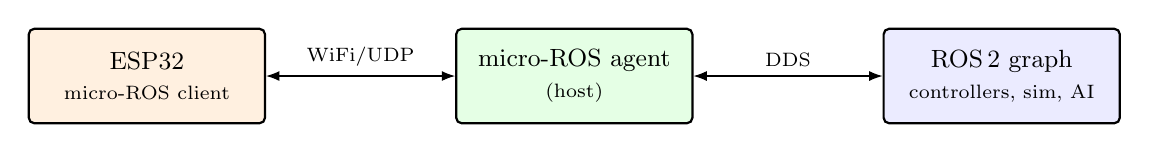
\begin{tikzpicture}[
      font=\small, >=Latex, node distance=20mm,
      b/.style={draw, rounded corners=2pt, align=center, thick,
                minimum height=12mm, minimum width=30mm},
    ]
    \node[b, fill=orange!12] (esp) {ESP32\\\scriptsize micro-ROS client};
    \node[b, fill=green!10, right=24mm of esp] (agent) {micro-ROS agent\\\scriptsize (host)};
    \node[b, fill=blue!8, right=24mm of agent] (ros) {ROS\,2 graph\\\scriptsize controllers, sim, AI};
    \draw[<->] (esp) -- node[above,font=\scriptsize]{WiFi/UDP} (agent);
    \draw[<->] (agent) -- node[above,font=\scriptsize]{DDS} (ros);
  \end{tikzpicture}
  \caption{micro-ROS bridges the microcontroller to the ROS\,2 graph: a
           lightweight client on the ESP32 talks to an agent on the host,
           which connects it to the full DDS network.}
  \label{fig:microros}
\end{figure}

This is exactly why micro-ROS is convenient here: the on-robot controller
speaks the same language as everything else, so the inertial data and the
joint commands are exposed as standard ROS\,2 topics, with no custom
protocol or translation glue to maintain. Concretely, the firmware
advertises a node that \emph{subscribes} to the joint-command topic and
\emph{publishes} the IMU topic. Both use \textbf{best-effort} delivery:
for a continuous stream of set-points and inertial samples, the newest
value always supersedes the previous one, so re-transmitting a lost
message would only add latency.

Because the wireless link can drop, the firmware tolerates an agent that
comes and goes through the explicit state machine of
Figure~\ref{fig:fsm}. It waits for the network, then for the agent; once
the agent answers it creates the ROS\,2 entities and enters the connected
state, where it periodically re-checks the link. If the agent is lost,
the node cleanly destroys its entities and returns to waiting --- so the
robot reconnects automatically, without a reboot. An on-board LED mirrors
this state, lit only while connected.

\begin{figure}[ht]
  \centering
  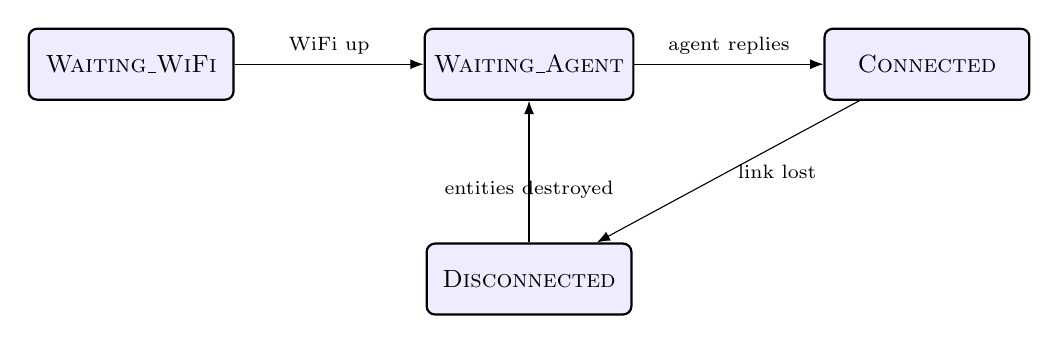
\begin{tikzpicture}[
      font=\small, >=Latex, node distance=18mm and 24mm,
      st/.style={draw, rounded corners=3pt, align=center, thick,
                 minimum height=9mm, minimum width=26mm, fill=blue!7}
    ]
    \node[st] (wifi) {\textsc{Waiting\_WiFi}};
    \node[st, right=of wifi] (agent) {\textsc{Waiting\_Agent}};
    \node[st, right=of agent] (conn) {\textsc{Connected}};
    \node[st, below=of agent] (disc) {\textsc{Disconnected}};

    \draw[->] (wifi) -- node[above,font=\scriptsize,align=center]{WiFi up} (agent);
    \draw[->] (agent) -- node[above,font=\scriptsize,align=center]{agent replies} (conn);
    \draw[->] (conn) -- node[right,font=\scriptsize,align=center]{link lost} (disc);
    \draw[->] (disc) -- node[below,font=\scriptsize,align=center]{entities destroyed} (agent);
  \end{tikzpicture}
  \caption{Agent-connection state machine, providing automatic
           reconnection without rebooting the robot.}
  \label{fig:fsm}
\end{figure}

\section{Conclusion}
This chapter described the embedded firmware of Abbes. The ESP32 was
chosen for its dual-core processing, integrated WiFi, native
I\textsuperscript{2}C support, and low cost. Around it, the firmware is
organised into focused modules running two periodic data paths --- a
100~Hz servo loop and a 50~Hz sensing loop --- with per-joint limiting
and velocity-limited interpolation to protect the hardware. The actuators
and the inertial sensor share a single I\textsuperscript{2}C bus, and the
node joins the rest of the system through micro-ROS, which makes the
microcontroller a first-class participant in the ROS\,2 graph. That graph
--- the host-side software architecture that produces the joint commands
and consumes the inertial data --- is the subject of the next chapter.


\end{document}
